Las simulaciones aceleradas fueron llevadas a cabo en el ensamble NVT a 300.0 K
con un termostato de Langevin ~\cite{schneider1978} utilizando una versión 
modificada de \path{GEMS} ~\cite{gems}. A cada estructura se le realizó una 
minimización de gradientes conjugados con el software \path{LAMMPS} 
~\cite{lammps1, lammps2}. El tamaño de los sistemas y la cantidad de estructuras 
utilizadas para obtener los siguiente resultados se presentan en la Tabla 
\ref{t:siminfo}.
\begin{table}[h]
    \centering
    \caption{Información del conjunto de datos.}
    \setlength\extrarowheight{2pt}\stackon{%
    \begin{tabular}{c c c c c c c}
        \toprule
        \textbf{$x$ en Li$_{x}$Si} & 
        \textbf{$N_{\text{Li}}$} & 
        \textbf{$N_{\text{Si}}$} &
        \textbf{$N_{\text{estructuras}}$} & 
        \textbf{$E$ / $N$ [eV]} \\ 
        \midrule
        0.21 & 140 & 667 & 774 & -4.399 $\pm$ 0.003 \\
        0.62 & 416 & 670 & 1665 & -4.002 $\pm$ 0.005 \\
        1.25 & 839 & 671 & 1224 & -3.521 $\pm$ 0.004 \\
        1.71 & 1152 & 672 & 2132 & -3.286 $\pm$ 0.002 \\
        2.17 & 693 & 319 & 1699 & -3.126 $\pm$ 0.002 \\
        2.71 & 865 & 319 & 1504 & -2.964 $\pm$ 0.002 \\
        3.25 & 1040 & 320 & 1464 & -2.856 $\pm$ 0.003 \\
        3.75 & 1080 & 288 & 2660 & -2.777 $\pm$ 0.002 \\
        4.20 & 1344 & 320 & 1600 & -2.717 $\pm$ 0.001 \\
        \bottomrule
    \end{tabular}
    }{}
    \label{t:siminfo}
\end{table}

\begin{figure}[h]
    \centering
    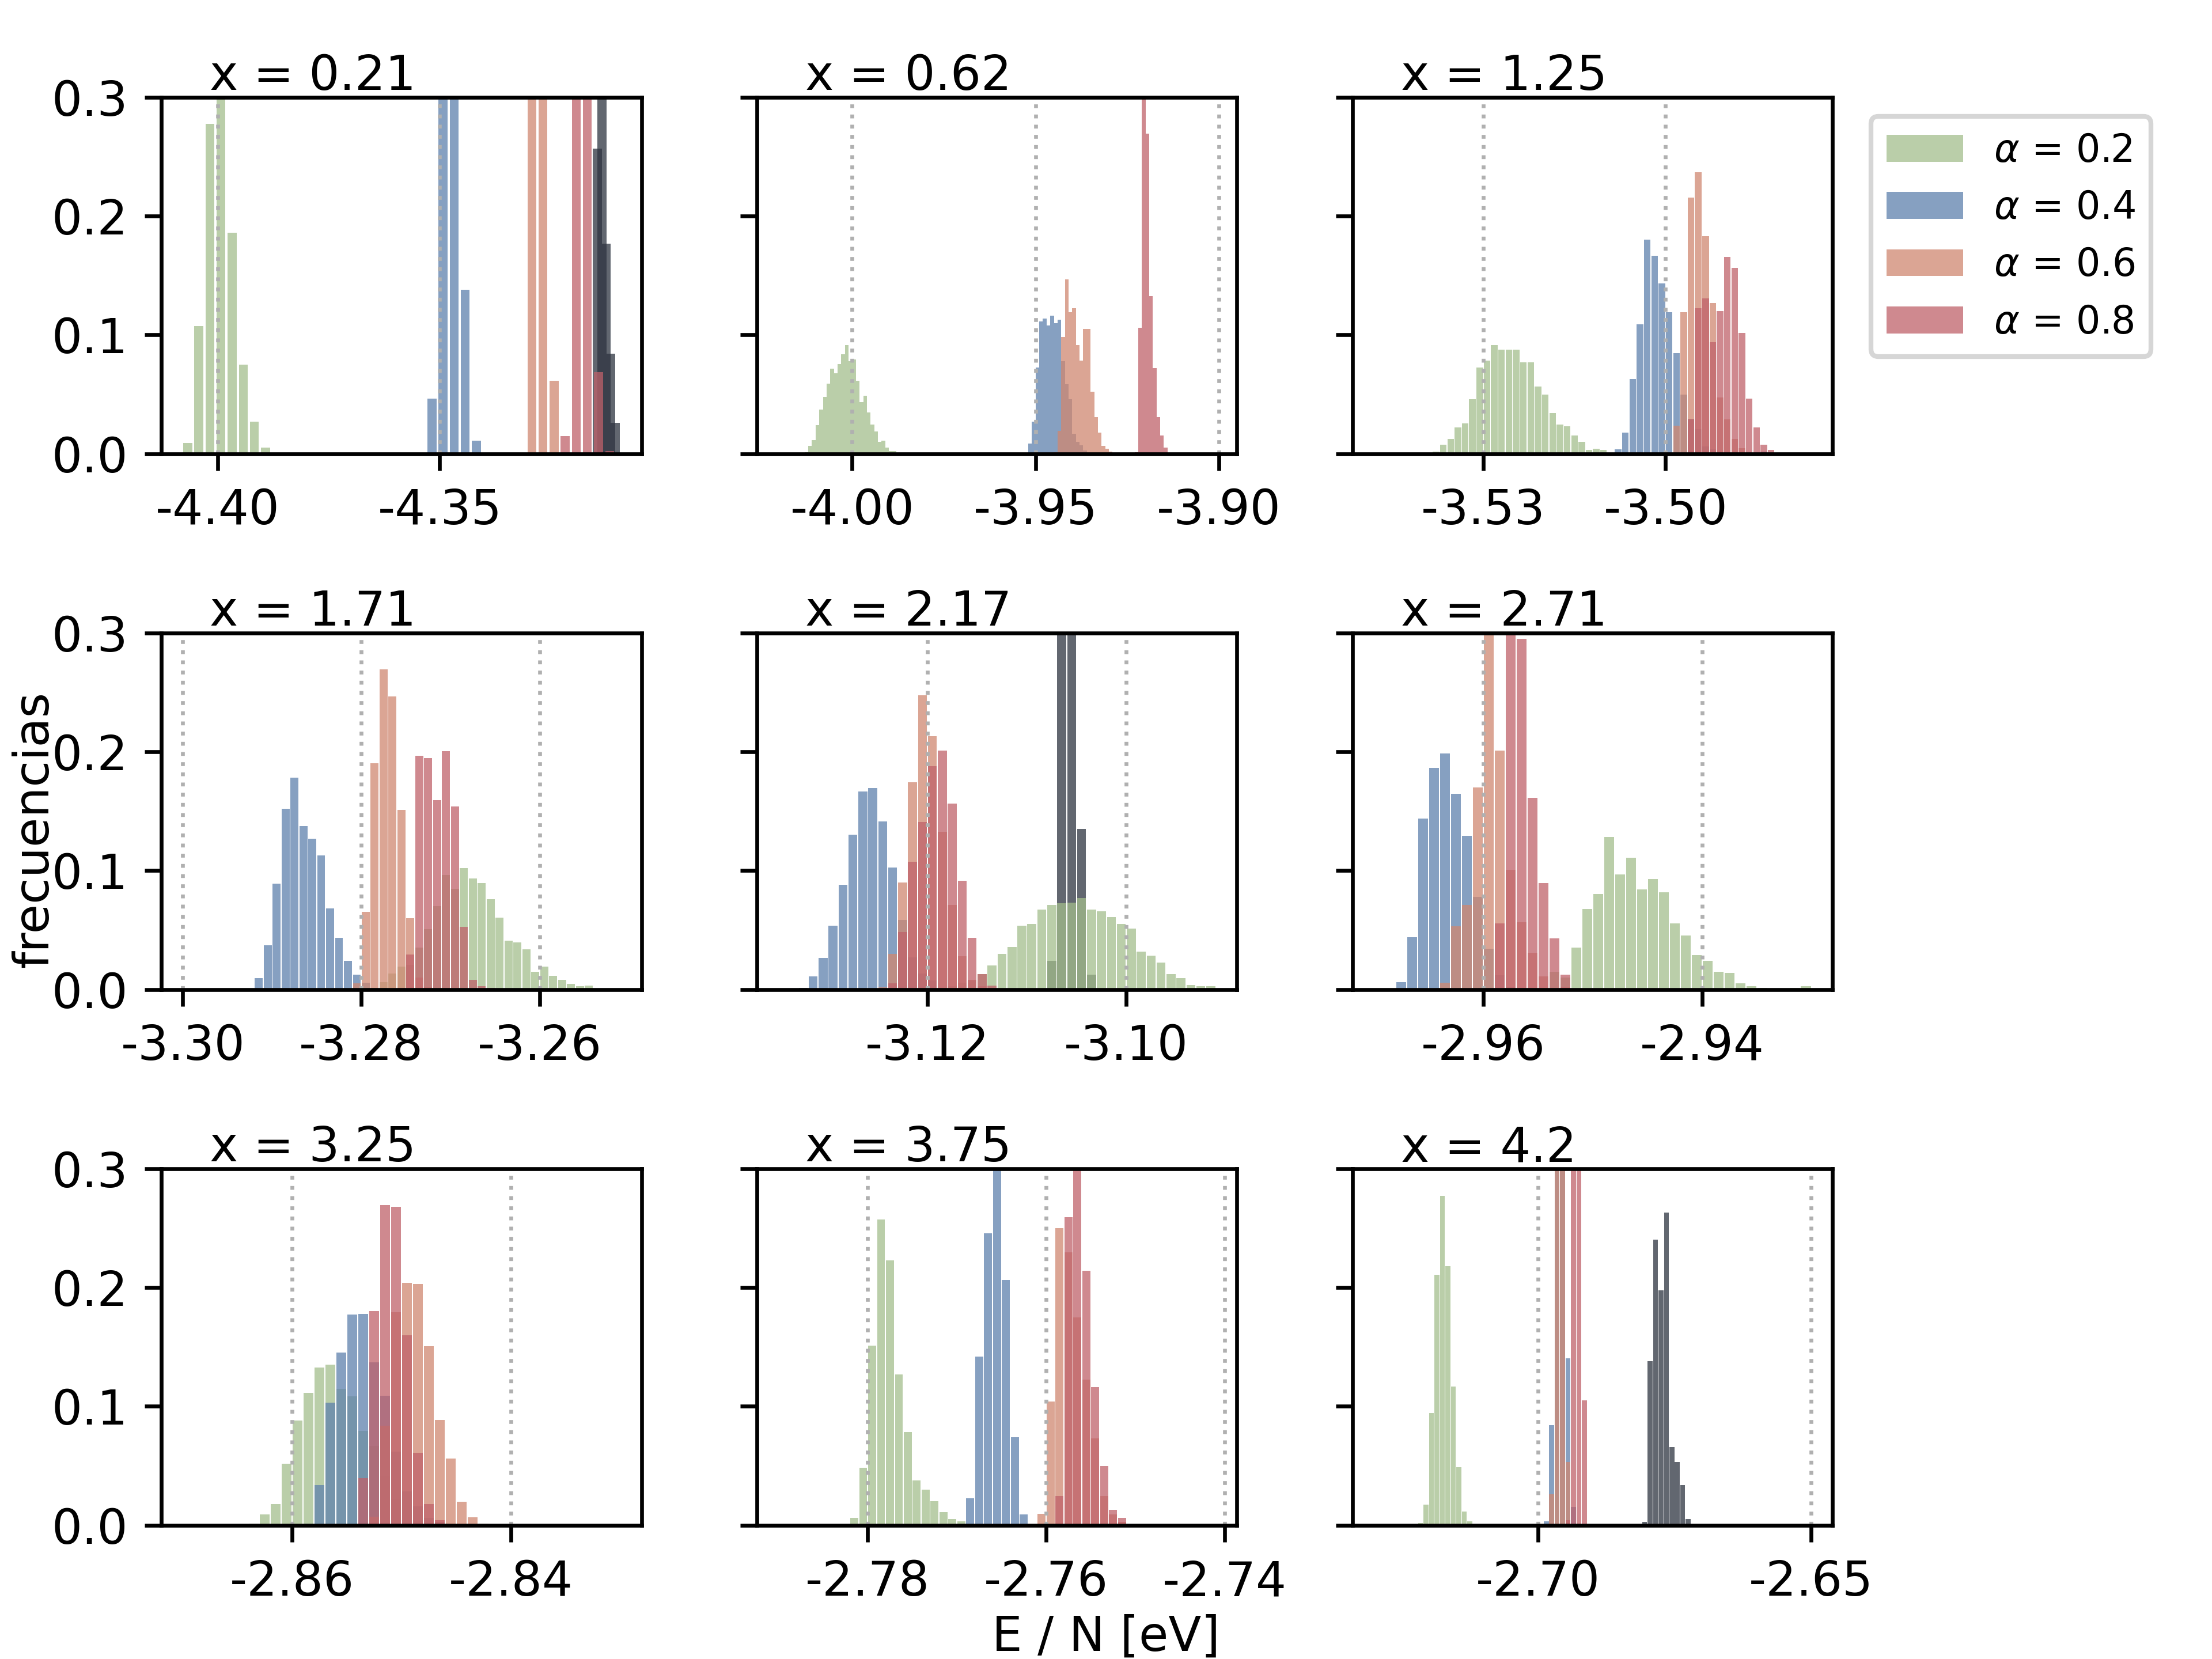
\includegraphics[width=\textwidth]{Silicio/caracterizacion/resultados/introduccion/energias.png}
    \caption{Histogramas correspondientes a la energía potencial de las 
    estructuras obtenidas con el método AELM, con distintos valores de $\alpha$
    en la ecuación \ref{eq:bias}, para cada composición de Li$_x$Si estudiada.}
    \label{fig:energias}
\end{figure}
La Figura \ref{fig:energias} muestra los histogramas para las energías mínimas
de las estructuras de Li$_x$Si obtenidas con el método AELM para los valores de
$x$ estudiados y distintos valores de compresión $\alpha$. En cada fila hay un 
histograma de energías representativo para las estructuras de concentración 
cercana, por lo cual en el análisis sólo son nombradas algunas de estas 
concentraciones. Para el primer caso, donde $x = 0.21$, se puede apreciar como el 
uso de valores más pequeños de $\alpha$ permite que estructuras con menor energía 
sean encontradas. El principal efecto de este factor $\alpha$ sobre la PES es la 
disminución de sus barreras de energía, mejorando la exploración del espacio de 
las fases. Este efecto se vuelve más drástico a medida que el valor de $\alpha$ 
tiende a cero. Para estas concentraciones representativas también se realizaron 
simulaciones de MD usuales, es decir, con un valor de $\alpha = 1$, estas no 
pueden sobrepasar las barreras de energías durante el tiempo simulado. El sistema 
permanece cercano al mínimo local asociado a la configuración inicial. Por otro 
lado, el uso de $\alpha = 0.2$ en el método de AELM resulta en un acceso rápido
a estructuras de energías menores. Un comportamiento similar se observa para 
$x = 2.17$, sin embargo, en este caso el valor más pequeño de $\alpha$ tiende a 
encontrar energías más altas que los otros casos, dando lugar a una distribución
similar a la de MD ordinaria pero con mayores fluctuaciones. Esto probablemente 
se deba a una exploración demasiado extensa, donde el sistema difunde a través
de una gran región del espacio de las fases y las minimizaciones múltiples de 
CG no son capaces de encontrar mínimos de menor energía. Por último, para la 
concentración más alta, correspondiente a un valor de $x = 4.2$, las simulaciones 
de AELM con un valor de $\alpha = 0.2$ son capaces de encontrar estructuras que 
reducen fuertemente la energía potencial del sistema. 

\begin{figure}[t]
    \centering
    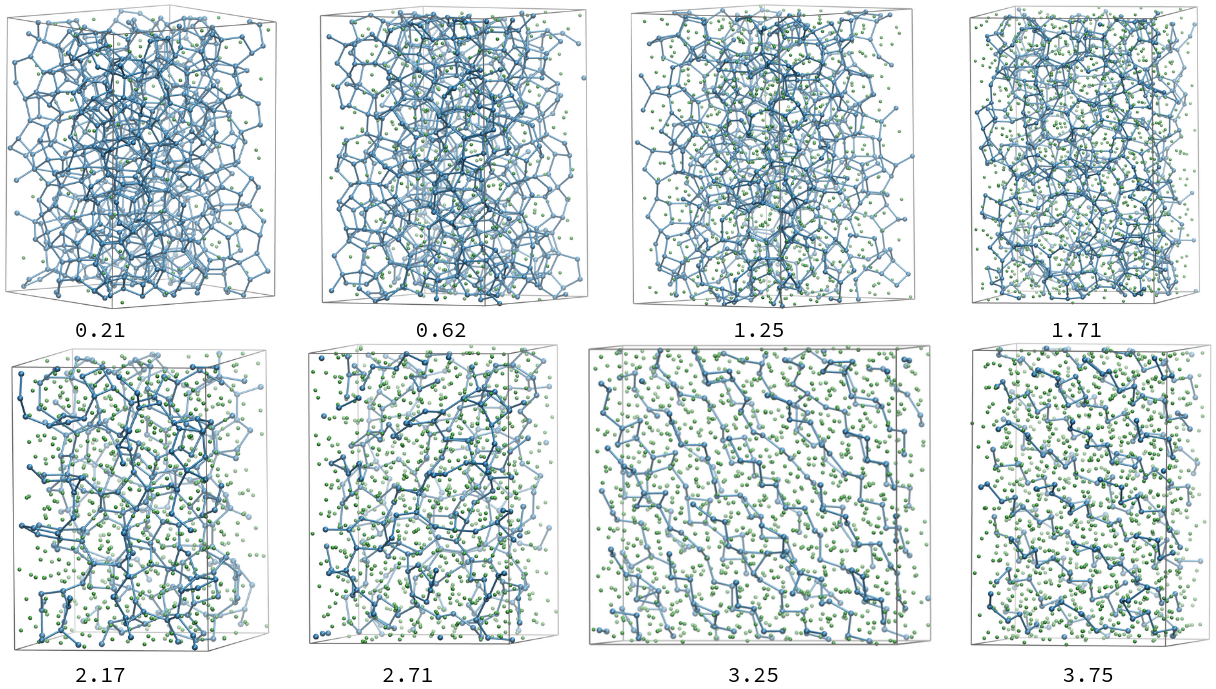
\includegraphics[width=\textwidth]{Silicio/caracterizacion/resultados/introduccion/amorfas.png}
    \caption{Configuración amorfa representativa de cada valor de $x$. Los átomos
    de Si se muestran en azul mientras que los de Li en verde.}
    \label{fig:amorfas}
\end{figure}
De los histogramas de la Figura \ref{fig:energias} se seleccionan los factores 
de aceleración más óptimos, es decir que producen energías menores, para obtener
las propiedades estructurales que se discuten a continuación. Para estos valores
se muestra una estructura representativa a cada composición en la Figura 
\ref{fig:amorfas}. Para $x = 0.21$ puede verse que la red amorfa de silicio
permanece con su estructura tetraédrica desordenada. Algunos enlaces Si-Si 
comienzan a romperse a medida que la concentración de litio aumenta, como puede
verse para las estructuras cercanas a $x = 2.17$. Por último, para las 
concentraciones más altas de litio, se alcanzan estructuras que involucran 
cadenas unidimensionales periódicas de silicio. Una estructura similar ha sido 
reportada por Ostadhossein \textit{et al.} ~\cite{ostadhossein2015}. En las 
próximas secciones se caracterizan dichas estructuras.
